\documentclass[border=6mm]{standalone}

\usepackage{tikz}
% \usepackage{tgheros}
\usepackage[sfdefault,scaled=.85]{FiraSans}
\usepackage{newtxsf}
\usepackage{microtype}

\begin{document}
Third Change

Test

Test 1

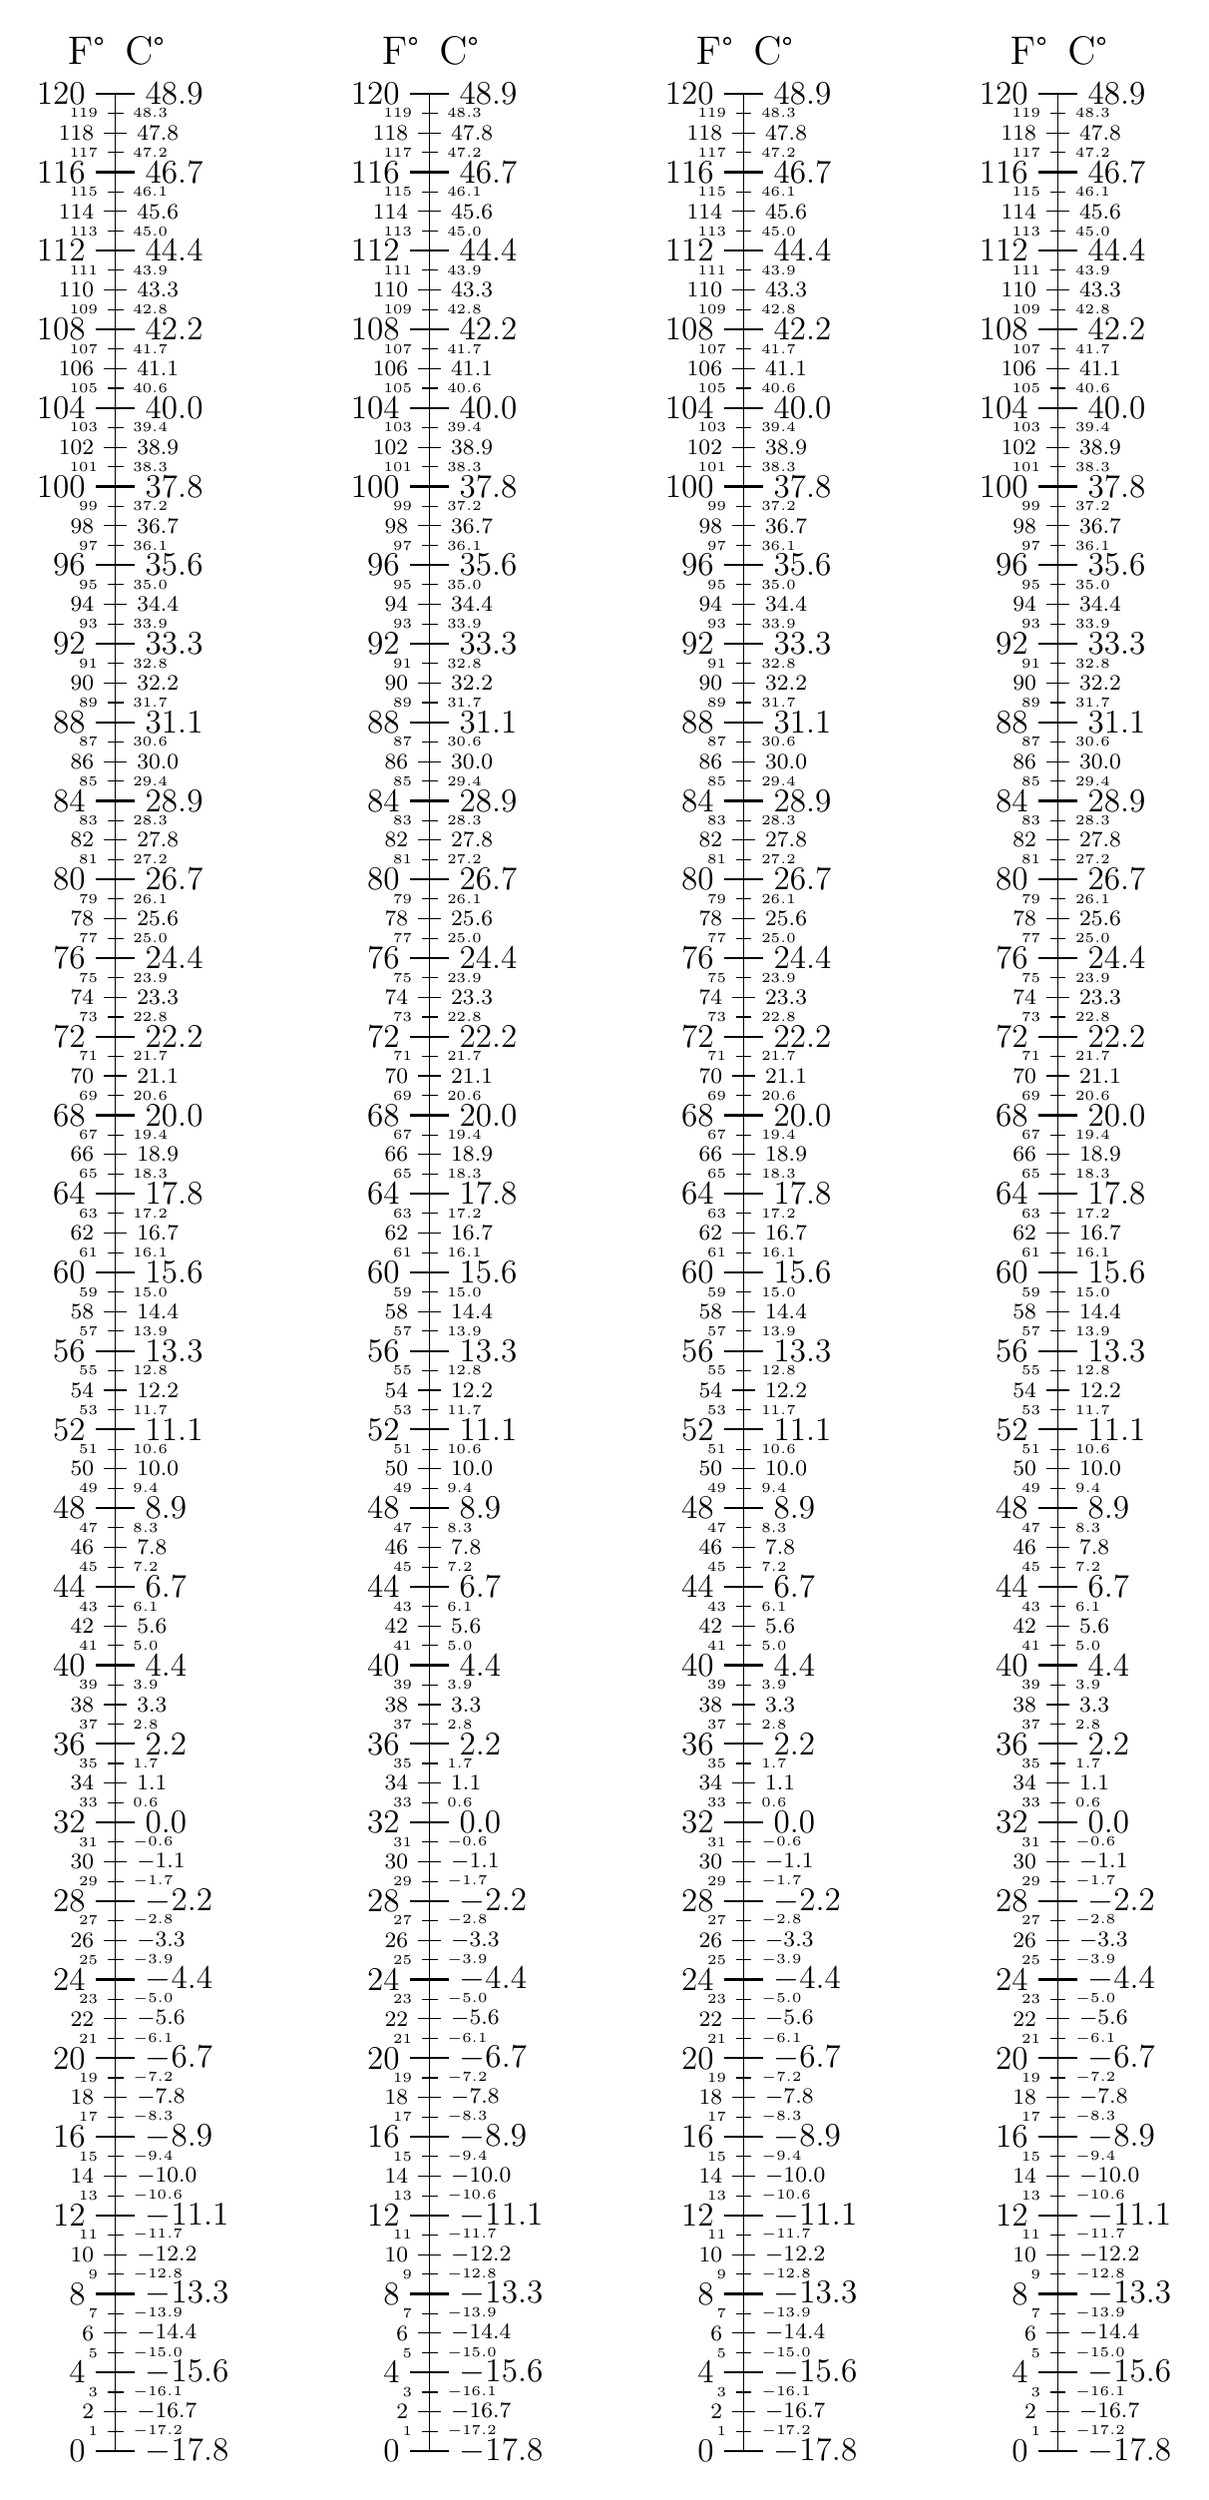
\begin{tikzpicture}[yscale=0.25]
  \foreach \j in {0,4, ..., 12} % positions for the four scales
  {
    % Start with Fahrenheit scale
    \pgfkeys{/pgf/number format/.cd,std,fixed,int detect,precision=0}
    \node[anchor=south east] at (\j ,121) {\Large {F\textdegree}};
    \draw (\j,0)-- (\j, 120); % draw the vertical axis   
    \foreach \i in {0,4,...,120} % numbers on line - major ticks
        \draw[thick] (\j,\i) -- + (-0.25,0) node[left]   {\large{\pgfmathprintnumber{\i}}};
    \foreach \i in {2,6,...,118} % numbers on line - minor ticks
        \draw (\j,\i) -- + (-0.15,0) node[left] {\footnotesize{\pgfmathprintnumber{\i}}};
    \foreach \i in {1,3,...,119} % numbers on line - minor-minor ticks
        \draw (\j,\i) -- + (-0.1,0) node[left] {\tiny{\pgfmathprintnumber{\i}}};

    % Proceed to Celsius scale
    \pgfkeys{/pgf/number format/.cd,std,fixed,zerofill=true,precision=1}
    \node[anchor=south west] at (\j ,121) {\Large{C\textdegree}};

    \foreach \i in {0,4,...,120} % numbers on line - major ticks
        \draw[thick] (\j,\i) -- + (0.25,0) node[right] {\large{\pgfmathparse{(\i-32)*5/9}\pgfmathprintnumber{\pgfmathresult}}};
    \foreach \i in {2,6,...,118} % numbers on line - minor ticks
        \draw (\j,\i) -- + (0.15,0) node[right] {\footnotesize{\pgfmathparse{(\i-32)*5/9}\pgfmathprintnumber{\pgfmathresult}}};
    \foreach \i in {1,3,...,119} % numbers on line - minor-minor ticks
        \draw (\j,\i) -- + (0.1,0) node[right] {\tiny{\pgfmathparse{(\i-32)*5/9}\pgfmathprintnumber{\pgfmathresult}}};
  }
  
\end{tikzpicture}
\end{document}

